\chapter{Neutron Partonic Structure}
\label{chap:physics}

\section{Physics motivations: Neutron GPDs}

Electromagnetic probes have played a major role in advancing our knowledge 
about the structure of the nucleon. While lepton-nucleon elastic scattering 
measurements have taught us about the spatial charge and magnetization 
distributions \cite{PhysRev.98.217,Perdrisat:2006hj}, deep-inelastic scattering experiments 
have uncovered the partonic structure of the nucleon and the longitudinal 
momentum distributions of the constituent partons, i.e., quarks and gluons 
\cite{PhysRevD.98.030001}.  With nuclear targets, deeply inelastic lepton scattering measurements 
have revealed that the distribution of quarks in a nucleus is not a simple 
convolution of their distributions within nucleons, an observation known as the 
``EMC effect''\cite{Aubert:1981gw} (for reviews on the topic, see  
\cite{ARNEODO1994301,Geesaman:1995yd,Norton:2003cb,RevModPhys.89.045002}).

A wealth of information on the structure of hadrons lies in the correlations 
between the momentum and spatial degrees of freedom of the partons. These 
correlations can be revealed through deeply virtual Compton scattering (DVCS), 
i.e., the hard exclusive lepto-production of a real photon, which provides 
access to a three-dimensional (3-D) imaging of partons within the generalized 
parton distributions (GPDs) framework 
\cite{Mueller:1998fv,PhysRevLett.78.610,PhysRevD.55.7114,Radyushkin:1996nd,PhysRevD.56.5524}.   
The measurement of free proton DVCS has been the focus of a worldwide effort 
\cite{PhysRevLett.87.182002,
   PhysRevLett.87.182001,
   PhysRevD.75.011103,
   Girod:2007aa,
   PhysRevC.92.055202,
   PhysRevLett.99.242501,
   PhysRevC.80.035206,
   PhysRevLett.114.032001,
   Jo:2015ema}
involving several accelerator facilities such as Jefferson Lab, DESY and  
CERN. These measurements now enable the extractions of GPDs and a 3-D 
tomography of the free proton \cite{Guidal:2013rya, PhysRevD.95.011501}. The 
aim of this proposal is enhance the neutron GPD measurements along the approved 
CLAS12 experiment E12-11-003, which will also measure the quasi-free neutron 
DVCS by detecting the scattered neutron in deuterium.  

\section{DVCS Formalism and Observables}

The cross section for DVCS on a spin-1/2 target can be parameterized in terms 
of four helicity conserving GPDs: $H^q$, $E^q$, $\tilde{H}^q$, and 
$\tilde{E}^q$. The GPDs $H$, $E$, $\widetilde{H}$ and $\widetilde{E}$ are 
defined for each quark flavor (q = u, d, s, ... ). Analogous GPDs exist for the 
gluons, see references \cite{PhysRevLett.78.610,PhysRevD.56.5524,Goeke:2001tz} for details.  In 
this work, we are mostly concerned by the valence quark region, in which the 
sea quarks and the gluons contributions do not dominate the DVCS scattering 
amplitude. The GPDs $H$ and $\widetilde{H}$ conserve the spin of the nucleon, 
while $E$ and $\widetilde{E}$ flip it. The $H$ and $E$ GPDs are called the 
unpolarized GPDs as they represent the sum over the different configurations of 
the quarks' helicities, whereas $\widetilde{H}$ and $\widetilde{E}$ are called 
the polarized GPDs because they are made up of the difference between the 
orientations of the quarks' helicities.




\begin{figure}
   \centering
   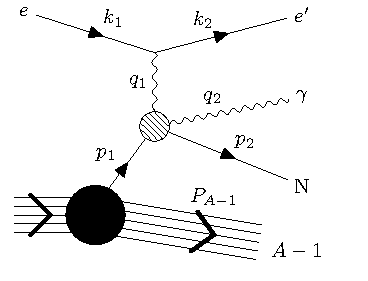
\includegraphics[width=0.60\textwidth]{figures/dvcs_feynman-figure5.pdf}
   \caption{\label{fig:dvcsMomenta}Incoherent DVCS process with the momentum 
   definitions labeled.}
\end{figure}

The DVCS cross section is written as
\begin{equation}
\frac{d\sigma}{dx_A\,dy\,dt\,d\phi\,d\varphi} = \frac{\alpha^3 x_A y}{16 \pi^2 
Q^2 \sqrt{1+\epsilon^2}} \left| \frac{\mathcal{T}}{e^3} \right|^2
\end{equation}
where
\begin{equation}
   \epsilon \equiv 2x_A \frac{M_A}{Q},
\end{equation}
$x_A=Q^2/(2p_1\cdot q_1$) is the scaling variable, $y= (p_1\cdot q_1)/(p_1\cdot 
k_1)$ is the photon energy fraction, $\phi$ is the angle between the leptonic 
and hadronic planes, $\varphi$ is the scattered electron's azimuthal angle, $Q^2= 
-q_1^2$, and $q_1=k_1-k_2$. The particle momentum definitions are shown in 
Figure~\ref{fig:dvcsMomenta}. We use the BMJ\footnote{The Belitsky, M\"{u}ller, and
Ji reference frame. See \cite{Braun:2014paa} for a nice discussion of the 
various reference frames.} 
convention~\cite{Braun:2014paa,Belitsky:2001ns,Belitsky:2010jw,Belitsky:2012ch} 
for defining the momentum transfer where the target nucleus is initially at 
rest, $\Delta = p_1-p_2$ and $t=\Delta^2$. The Bjorken variable  is related to 
the scaling variable by
%
\begin{equation}
   x_{\text{B}} = \frac{Q^2}{2 M_N E\,y} \simeq A x_A
\end{equation}
%
where $M_N$ is the nucleon mass and $E$ is the beam energy. Another scaling variable called skewedness is
%
\begin{equation}
\xi = \frac{x_A}{2 - x_A} + \mathcal{O}(1/Q^2)
\end{equation}
where the power suppressed contributions originate with the selection of the 
BMJ frame convention needed to unambiguously define the leading-twist 
approximation used in this proposal~\cite{Braun:2014paa}.

The amplitude is the sum of the DVCS and Bethe-Heitler (BH) amplitudes, and 
when squared has terms
\begin{equation}
   \mathcal{T}^2 = \left|\mathcal{T}_{\text{BH}}\right|^2 + 
   \left|\mathcal{T}_{\text{DVCS}}\right|^2 + \mathcal{I}
\end{equation}
where the first is the BH contribution, the second is the DVCS part, and the last 
term is the interference part,
\begin{equation}
   \mathcal{I} = \mathcal{T}_{\text{DVCS}}\mathcal{T}_{\text{BH}}^{*} + 
   \mathcal{T}_{\text{DVCS}}^{*}\mathcal{T}_{\text{BH}}.
\end{equation}
The corresponding amplitudes are calculated with the diagrams shown in 
Figure~\ref{fig:DVCShandbag}. The details of contracting the DVCS tensor with 
various currents and tensors can be found in~\cite{Kirchner:2003wt}.
\begin{figure}[!hbt]
   \centering
   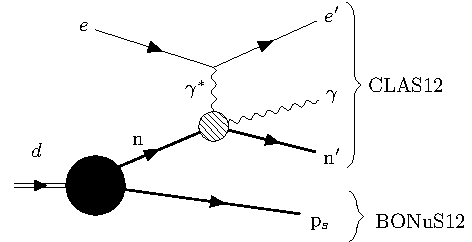
\includegraphics[width=0.20\textwidth]{figures/dvcs_feynman-figure1.pdf}
   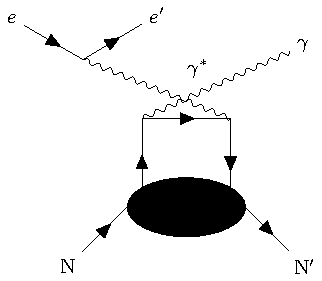
\includegraphics[width=0.20\textwidth]{figures/dvcs_feynman-figure2.pdf}
   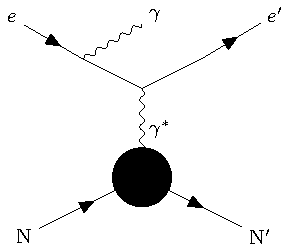
\includegraphics[width=0.20\textwidth]{figures/dvcs_feynman-figure3.pdf}
   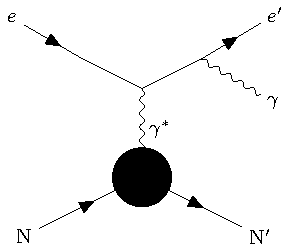
\includegraphics[width=0.20\textwidth]{figures/dvcs_feynman-figure4.pdf}
   \caption{\label{fig:DVCShandbag}DVCS handbag diagram and BH contributions 
   used for calculating DVCS amplitudes.}
\end{figure}
%
The resulting expressions for the amplitudes are
\begin{align}
   \left|\mathcal{T}_{\text{BH}}\right|^2 &= 
   \frac{e^6(1+\epsilon^2)^{-2}}{x_A^2\,y^2\,t\,
   \mathcal{P}_1(\phi)\mathcal{P}_2(\phi)} \left\{ c_0^{\text{BH}} + 
   \sum_{n=1}^{2}\left[ c_n^{\text{BH}}\cos(n\phi) +s_n^{\text{BH}}\cos(n\phi) 
\right] \right\} \\
\left|\mathcal{T}_{\text{DVCS}}\right|^2 &= \frac{e^6}{y^2\,Q^2}\left\{ 
c_0^{\text{DVCS}} + \sum_{n=1}^{2}\left[ c_n^{\text{DVCS}}\cos(n\phi) 
+s_n^{\text{DVCS}}\cos(n\phi) \right] \right\}\\
   \mathcal{I} &= \frac{e^6(1+\epsilon^2)^{-2}}{x_A\,y^3\,t\,
   \mathcal{P}_1(\phi)\mathcal{P}_2(\phi)}\left\{ c_0^{\mathcal{I}} + 
   \sum_{n=1}^{3}\left[ c_n^{\mathcal{I}}\cos(n\phi) 
+s_n^{\mathcal{I}}\cos(n\phi) \right] \right\}
\end{align}
%
The functions $c_0$, $c_n$, and $s_n$ are called \emph{Fourier coefficients} 
and they depend on the kinematic variables and the operator decomposition of 
the DVCS tensor for a target with a given spin. At leading twist there is a 
straightforward form factor decomposition which relates the vector and 
axial-vector operators with the so-called Compton form factors 
(CFFs)~\cite{Belitsky:2000gz}. The Compton form factors appearing in the DVCS 
amplitudes are integrals of the type
%
%
\begin{equation}
   \mathcal{F} = \int_{-1}^{1} dx F(\mp x,\xi,t) C^{\pm}(x,\xi)
\end{equation}
where the coefficient functions at leading order take the form
\begin{equation}
   C^{\pm}(x,\xi) = \frac{1}{x-\xi + i\epsilon} \pm \frac{1}{x+\xi - 
   i\epsilon}.
\end{equation}
%
We plan on measuring the beam spin asymmetry as a function of $\phi$
\begin{equation}
   A_{LU}(\phi) = \frac{d\sigma^{\uparrow}(\phi) - 
   d\sigma^{\downarrow}(\phi)}{d\sigma^{\uparrow}(\phi) + 
   d\sigma^{\downarrow}(\phi)}
\end{equation}
%
where the arrows indicate the electron beam helicity. 

\section{Tagged neutron DVCS with BONuS12}


\section{Fully exclusive neutron DVCS with BONuS12}





